%%%%%%%%%%%%%%%%%%%%%%%%%%%%%%%%%%%%%%%%%%%%%%%%%%%%%%%%%%%%%%%%%%%%%%%%%%%
%% This file is part of the book
%%
%% Algorithmic Graph Theory
%% http://code.google.com/p/graph-theory-algorithms-book/
%%
%% Copyright (C) 2009, 2010 Minh Van Nguyen <nguyenminh2@gmail.com>
%%
%% See the file COPYING for copying conditions.
%%%%%%%%%%%%%%%%%%%%%%%%%%%%%%%%%%%%%%%%%%%%%%%%%%%%%%%%%%%%%%%%%%%%%%%%%%%

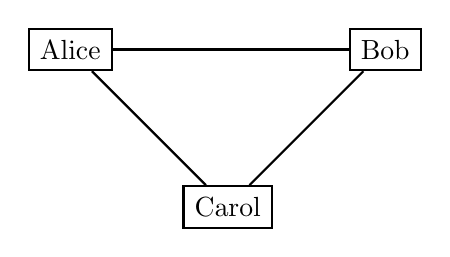
\begin{tikzpicture}
[nodedecorate/.style={shape=rectangle,inner sep=4pt,draw,thick},%
 linedecorate/.style={-,thick}]
%% nodes or vertices
\foreach \nodename/\x/\y in {Alice/-2/2, Bob/2/2, Carol/0/0} {
  \node (\nodename) at (\x,\y) [nodedecorate] {\nodename};
}
%% edges or lines
\path
\foreach \startnode/\endnode in {Alice/Bob, Alice/Carol, Bob/Carol} {
  (\startnode) edge[linedecorate] node {} (\endnode)
};
\end{tikzpicture}
